\documentclass[tikz,border=5pt]{standalone}
\usepackage{fontspec}
\setmainfont{Times New Roman}
\usepackage{unicode-math}
\setmathfont{Cambria Math}
\usetikzlibrary{shapes.geometric,positioning,fit,backgrounds,arrows.meta,calc}

\begin{document}
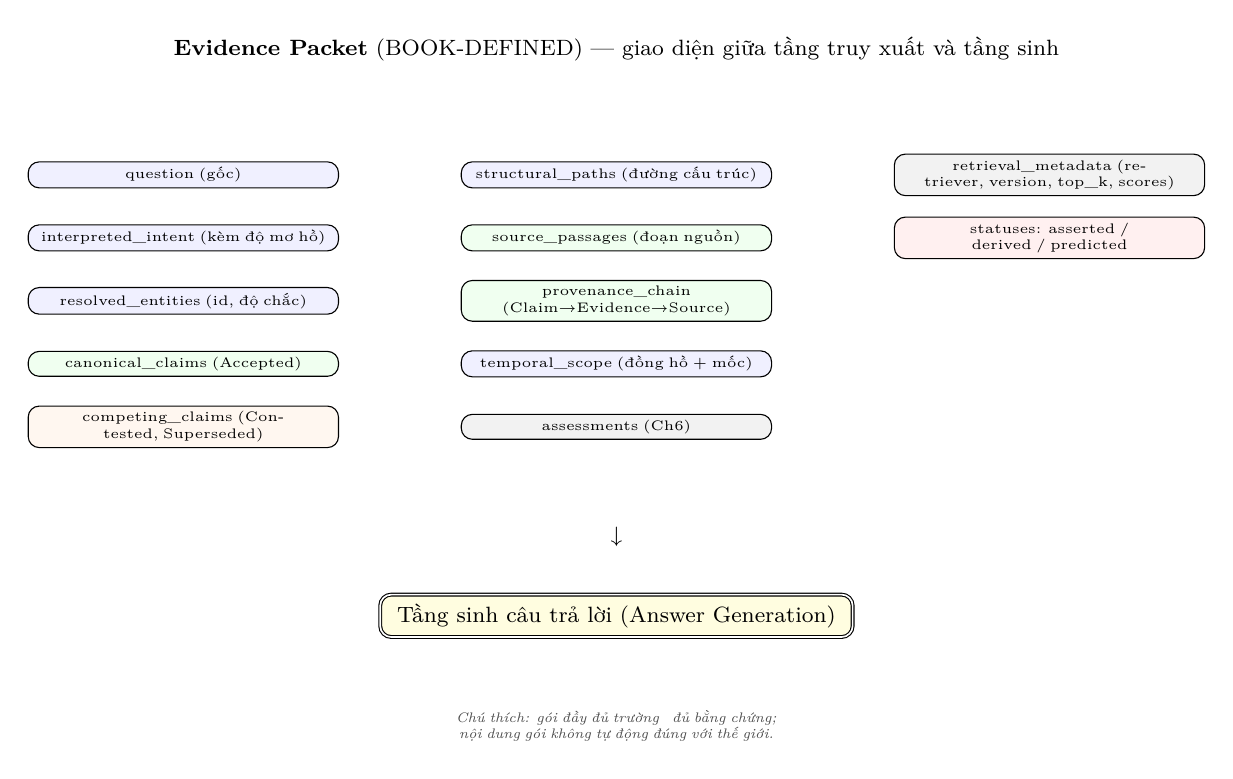
\begin{tikzpicture}[
  field/.style={rectangle, draw, rounded corners, fill=gray!6, align=center, font=\tiny, inner sep=2pt},
  label/.style={font=\tiny\itshape, text=gray!60!black},
  arrow/.style={-{Stealth[length=1.8mm]}, thin},
]

\node[font=\footnotesize, align=center] at (0, 5.6) {\textbf{Evidence Packet} (BOOK-DEFINED) — giao diện giữa tầng truy xuất và tầng sinh};

% Column 1
\node[field, text width=3.8cm, fill=blue!6] (f1) at (-5.5, 4) {question (gốc)};
\node[field, text width=3.8cm, fill=blue!6] (f2) at (-5.5, 3.2) {interpreted\_intent (kèm độ mơ hồ)};
\node[field, text width=3.8cm, fill=blue!6] (f3) at (-5.5, 2.4) {resolved\_entities (id, độ chắc)};
\node[field, text width=3.8cm, fill=green!6] (f4) at (-5.5, 1.6) {canonical\_claims (Accepted)};
\node[field, text width=3.8cm, fill=orange!6] (f5) at (-5.5, 0.8) {competing\_claims (Contested, Superseded)};

% Column 2
\node[field, text width=3.8cm, fill=blue!6] (f6) at (0, 4) {structural\_paths (đường cấu trúc)};
\node[field, text width=3.8cm, fill=green!6] (f7) at (0, 3.2) {source\_passages (đoạn nguồn)};
\node[field, text width=3.8cm, fill=green!6] (f8) at (0, 2.4) {provenance\_chain (Claim→Evidence→Source)};
\node[field, text width=3.8cm, fill=blue!6] (f9) at (0, 1.6) {temporal\_scope (đồng hồ + mốc)};
\node[field, text width=3.8cm, fill=gray!10] (f10) at (0, 0.8) {assessments (Ch6)};

% Column 3
\node[field, text width=3.8cm, fill=gray!10] (f11) at (5.5, 4) {retrieval\_metadata (retriever, version, top\_k, scores)};
\node[field, text width=3.8cm, fill=red!6] (f12) at (5.5, 3.2) {statuses: asserted / derived / predicted};

% Flow arrows
\node[font=\footnotesize, align=center] at (0, -0.6) {↓};
\node[draw, double, rounded corners, fill=yellow!12, minimum width=6cm, font=\footnotesize, align=center] (gen) at (0, -1.6) {Tầng sinh câu trả lời (Answer Generation)};

\node[label, align=center, text width=10cm] at (0, -3.0)
  {Chú thích: gói đầy đủ trường ≠ đủ bằng chứng;\\nội dung gói không tự động đúng với thế giới.};

\end{tikzpicture}
\end{document}